% -----------------------------------
% -----------------------------------
% abnTeX2: Normas ABNT NBR 14724:2011 + sugestões FGV/EMAp. 

% Autor: Lauro César Araujo
% Adaptações EMAp: Lucas Machado Moschen 
% Copyright 2012-2018 by abnTeX2 group at http://www.abntex.net.br/ 

%% This work may be distributed and/or modified under the
%% conditions of the LaTeX Project Public License, either version 1.3
%% of this license or (at your option) any later version.
%% The latest version of this license is in
%%   http://www.latex-project.org/lppl.txt
%% and version 1.3 or later is part of all distributions of LaTeX
%% version 2005/12/01 or later.
% ----------------------------------
% ----------------------------------
\documentclass[
	% -- opções da classe memoir --
	12pt,				% tamanho da fonte
	%openright,			% capítulos começam em página ímpar (insere página vazia caso preciso)
	oneside,			% para impressão em recto e verso. Oposto a oneside
	a4paper,			% tamanho do papel. 
	% -- opções da classe abntex2 --
	%chapter=TITLE,		% títulos de capítulos convertidos em letras maiúsculas
	%section=TITLE,		% títulos de seções convertidos em letras maiúsculas
	%subsection=TITLE,	% títulos de subseções convertidos em letras maiúsculas
	%subsubsection=TITLE,% títulos de subsubseções convertidos em letras maiúsculas
	% -- opções do pacote babel --
	english,			% idioma para inglês
	brazil				% idioma para português
	]{abntex2}

%------------------------------------------------
%-------------- Pacotes necessários -------------
%------------------------------------------------

% Escrita 
\usepackage[T1]{fontenc}
\usepackage[utf8]{inputenc}
\usepackage{lmodern}
\usepackage{microtype} % para melhorias de justificação
\usepackage{indentfirst}

\renewcommand{\ABNTEXchapterfont}{\fontfamily{ptm}\fontseries{b}\selectfont}

% Gráficos 
\usepackage{color}
\usepackage{caption}
\usepackage{subcaption}
\usepackage{graphicx}
\graphicspath{{../../images/}}
\usepackage{xcolor}

% Matemáticos 
\usepackage{amsthm, amssymb, amsmath, mathtools}

% Outros 
\usepackage{lipsum}
\usepackage{listings}
\usepackage{minted}


% Citações 
%\usepackage[brazilian,hyperpageref]{backref}
%\usepackage[alf]{abntex2cite}	% Citações padrão ABNT
\usepackage[style=abnt]{biblatex}
\addbibresource{biblio.bib}  

% \renewcommand{\backrefpagesname}{Citado na(s) página(s):~}
% % Texto padrão antes do número das páginas
% \renewcommand{\backref}{}
% % Define os textos da citação
% \renewcommand*{\backrefalt}[4]{
% 	\ifcase #1 %
% 		Nenhuma citação no texto.%
% 	\or
% 		Citado na página #2.%
% 	\else
% 		Citado #1 vezes nas páginas #2.%
% 	\fi}%
% ---


% Configurações do listings


\definecolor{lightgray}{rgb}{.9,.9,.9}
\definecolor{darkgray}{rgb}{.4,.4,.4}
\definecolor{purple}{rgb}{0.65, 0.12, 0.82}

\lstdefinelanguage{Python}{
  keywords={typeof, True, False, try, except, return, None, catch, var, if, in, while, do, else, case, break, elif, for, def, class, import},
  keywordstyle=\color{blue}\bfseries,
  ndkeywords={class, export, bool, raise, import, self, def},
  ndkeywordstyle=\color{darkgray}\bfseries,
  identifierstyle=\color{black},
  sensitive=false,
  comment=[l]{\#},
  morecomment=[s]{"""}{"""},
  commentstyle=\color{green}\ttfamily,
  stringstyle=\color{red}\ttfamily,
  morestring=[b]',
  morestring=[b]",
  escapeinside={\%*}{*)},
   literate=  {á}{{\'a}}1 {é}{{\'e}}1 {í}{{\'i}}1 {ó}{{\'o}}1 {ú}{{\'u}}1
  {Á}{{\'A}}1 {É}{{\'E}}1 {Í}{{\'I}}1 {Ó}{{\'O}}1 {Ú}{{\'U}}1
  {à}{{\`a}}1 {è}{{\`e}}1 {ì}{{\`i}}1 {ò}{{\`o}}1 {ù}{{\`u}}1
  {À}{{\`A}}1 {È}{{\'E}}1 {Ì}{{\`I}}1 {Ò}{{\`O}}1 {Ù}{{\`U}}1
  {ä}{{\"a}}1 {ë}{{\"e}}1 {ï}{{\"i}}1 {ö}{{\"o}}1 {ü}{{\"u}}1
  {Ä}{{\"A}}1 {Ë}{{\"E}}1 {Ï}{{\"I}}1 {Ö}{{\"O}}1 {Ü}{{\"U}}1
  {â}{{\^a}}1 {ê}{{\^e}}1 {î}{{\^i}}1 {ô}{{\^o}}1 {û}{{\^u}}1
  {Â}{{\^A}}1 {Ê}{{\^E}}1 {Î}{{\^I}}1 {Ô}{{\^O}}1 {Û}{{\^U}}1
  {ç}{{\c c}}1 {Ç}{{\c C}}1 {ø}{{\o}}1 {å}{{\r a}}1 {Å}{{\r A}}1
  {ã}{{\~a}}1 {Ã}{{\~A}}1 {õ}{{\~o}}1 {Õ}{{\~O}}1
}

\lstdefinelanguage{Stata}{
  keywords={quietly, infix, byte, using, clear, format, \%, label, var, define, add, values},
  keywordstyle=\color{blue}\bfseries,
  ndkeywords={class, export, bool, raise, import, self, def},
  ndkeywordstyle=\color{darkgray}\bfseries,
  identifierstyle=\color{black},
  sensitive=false,
  comment=[l]{*},
  %morecomment=[s]{"""}{"""},
  commentstyle=\color{green}\ttfamily,
  stringstyle=\color{red}\ttfamily,
  %morestring=[b]',
  morestring=[b]",
  escapeinside={\%*}{*)},
   literate=  {á}{{\'a}}1 {é}{{\'e}}1 {í}{{\'i}}1 {ó}{{\'o}}1 {ú}{{\'u}}1
  {Á}{{\'A}}1 {É}{{\'E}}1 {Í}{{\'I}}1 {Ó}{{\'O}}1 {Ú}{{\'U}}1
  {à}{{\`a}}1 {è}{{\`e}}1 {ì}{{\`i}}1 {ò}{{\`o}}1 {ù}{{\`u}}1
  {À}{{\`A}}1 {È}{{\'E}}1 {Ì}{{\`I}}1 {Ò}{{\`O}}1 {Ù}{{\`U}}1
  {ä}{{\"a}}1 {ë}{{\"e}}1 {ï}{{\"i}}1 {ö}{{\"o}}1 {ü}{{\"u}}1
  {Ä}{{\"A}}1 {Ë}{{\"E}}1 {Ï}{{\"I}}1 {Ö}{{\"O}}1 {Ü}{{\"U}}1
  {â}{{\^a}}1 {ê}{{\^e}}1 {î}{{\^i}}1 {ô}{{\^o}}1 {û}{{\^u}}1
  {Â}{{\^A}}1 {Ê}{{\^E}}1 {Î}{{\^I}}1 {Ô}{{\^O}}1 {Û}{{\^U}}1
  {ç}{{\c c}}1 {Ç}{{\c C}}1 {ø}{{\o}}1 {å}{{\r a}}1 {Å}{{\r A}}1
  {ã}{{\~a}}1 {Ã}{{\~A}}1 {õ}{{\~o}}1 {Õ}{{\~O}}1
}

\lstset{
   %backgroundcolor=\color{lightgray},
   extendedchars=true,
   %basicstyle=\footnotesize\ttfamily,
   showstringspaces=false,
   showspaces=false,
   %numbers=left,
   %numberstyle=\footnotesize,
   numbersep=9pt,
   tabsize=2,
   breaklines=true,
   showtabs=false,
   captionpos=b,
   escapeinside={\%*}{*)},
   literate=  {á}{{\'a}}1 {é}{{\'e}}1 {í}{{\'i}}1 {ó}{{\'o}}1 {ú}{{\'u}}1
  {Á}{{\'A}}1 {É}{{\'E}}1 {Í}{{\'I}}1 {Ó}{{\'O}}1 {Ú}{{\'U}}1
  {à}{{\`a}}1 {è}{{\`e}}1 {ì}{{\`i}}1 {ò}{{\`o}}1 {ù}{{\`u}}1
  {À}{{\`A}}1 {È}{{\'E}}1 {Ì}{{\`I}}1 {Ò}{{\`O}}1 {Ù}{{\`U}}1
  {ä}{{\"a}}1 {ë}{{\"e}}1 {ï}{{\"i}}1 {ö}{{\"o}}1 {ü}{{\"u}}1
  {Ä}{{\"A}}1 {Ë}{{\"E}}1 {Ï}{{\"I}}1 {Ö}{{\"O}}1 {Ü}{{\"U}}1
  {â}{{\^a}}1 {ê}{{\^e}}1 {î}{{\^i}}1 {ô}{{\^o}}1 {û}{{\^u}}1
  {Â}{{\^A}}1 {Ê}{{\^E}}1 {Î}{{\^I}}1 {Ô}{{\^O}}1 {Û}{{\^U}}1
  {œ}{{\oe}}1 {Œ}{{\OE}}1 {æ}{{\ae}}1 {Æ}{{\AE}}1 {ß}{{\ss}}1
  {ç}{{\c c}}1 {Ç}{{\c C}}1 {ø}{{\o}}1 {å}{{\r a}}1 {Å}{{\r A}}1
  {€}{{\EUR}}1 {£}{{\pounds}}1 {ã}{{\~a}}1,
   frame=lines,
   numberbychapter=false
}

\lstloadlanguages{Python, Stata}







%----------------------------------------
%------- Capa e Folha de Rosto ----------
%----------------------------------------

\newcommand\subtitulo[1]{\def\@subtitulo{#1}}
%\newcommand{\imprimirsubtitulo}{\@subtitulo}

\renewcommand{\imprimircapa}{%
	\begin{capa}%
	\center
		\ABNTEXchapterfont\Large \MakeUppercase{\imprimirinstituicao}
		\\\vspace*{4cm}
		{\ABNTEXchapterfont\large \MakeUppercase{\imprimirautor}}
		\vfill
		\begin{center}
		\ABNTEXchapterfont\large\MakeUppercase{\imprimirtitulo}\normalfont\MakeUppercase{
		\imprimirsubtitulo}
		\end{center}
		\vfill
		\normalfont\large\imprimirlocal
		\\\normalfont\large\imprimirdata
		\vspace*{1cm}
	\end{capa}
}

\makeatletter
\renewcommand{\folhaderostocontent}{
  \begin{center}

    %\vspace*{1cm}
    {\ABNTEXchapterfont\large\MakeUppercase{\imprimirautor}}
	
    \vspace*{\fill}\vspace*{\fill}
    \begin{center}
      \ABNTEXchapterfont\bfseries\large\MakeUppercase{\imprimirtitulo}\normalfont\MakeUppercase{
      \imprimirsubtitulo}
    \end{center}
    \vspace*{\fill}
	
    \abntex@ifnotempty{\imprimirpreambulo}{%
      \hspace{7.5cm}
      \begin{minipage}{.5\textwidth}
      	\SingleSpacing
         \imprimirpreambulo
         \\\\
         Orientador: \imprimirorientador
       \end{minipage}%
       \vspace*{\fill}
    }%

    % {\large\imprimirorientadorRotulo~\imprimirorientador\par}
    % \abntex@ifnotempty{\imprimircoorientador}{%
    %    {\large\imprimircoorientadorRotulo~\imprimircoorientador}%
    % }%
    \vspace*{\fill}

    {\large\imprimirlocal}
    \par
    {\large\imprimirdata}
    \vspace*{1cm}

  \end{center}
}
\makeatother

\titulo{DESENVOLVIMENTO DE UM REPOSITÓRIO UNIFICADO DE DADOS PÚBLICOS}
\autor{Gianlucca Devigili}
\local{Rio de Janeiro}
\data{2023}
\instituicao{%
  Fundação Getulio Vargas \\
  \par
  Escola de Matemática Aplicada
}
\tipotrabalho{Trabalho de Conclusão de Curso}

\preambulo{Trabalho de conclusão de curso apresentada para a Escola de
Matemática Aplicada (FGV/EMAp) como requisito para o grau de bacharel em
Ciência de Dados e Inteligência Artificial. \\ \\ Área de estudo: ciência de dados.}

\orientador{Júlio César Chaves}

% Se o seu texto tem subtítulo. 
% Se não tiver, altere o arquivo capa_folha_rosto_tex
%\subtitulo{Este é o subtítulo do meu TCC}

%---------------------------------------------
%-------------------- PDF --------------------
%---------------------------------------------

% alterando o aspecto da cor azul
\definecolor{blue}{RGB}{41,5,195}

% informações do PDF
\makeatletter
\hypersetup{
     	%pagebackref=true,
		pdftitle={\@title}, 
		pdfauthor={\@author},
    	pdfsubject={\imprimirpreambulo},
	    pdfcreator={LaTeX with abnTeX2},
		pdfkeywords={abnt}{latex}{abntex}{abntex2}{trabalho acadêmico}, 
		colorlinks=true,       		% false: boxed links; true: colored links
    	linkcolor=blue,          	% color of internal links
    	citecolor=blue,        		% color of links to bibliography
    	filecolor=magenta,      		% color of file links
		urlcolor=blue,
		bookmarksdepth=4
}
\makeatother

% Posiciona figuras e tabelas no topo da página quando adicionadas sozinhas
% em um página em branco. Ver https://github.com/abntex/abntex2/issues/170
\makeatletter
\setlength{\@fptop}{5pt} % Set distance from top of page to first float
\makeatother

%---------------------------------------
%--------- Mais configurações-----------
%---------------------------------------

% Possibilita criação de Quadros e Lista de quadros.
% Ver https://github.com/abntex/abntex2/issues/176
\newcommand{\quadroname}{Quadro}
\newcommand{\listofquadrosname}{Lista de quadros}

% \newfloat[chapter]{quadro}{loq}{\quadroname}
\newlistof{listofquadros}{loq}{\listofquadrosname}
\newlistentry{quadro}{loq}{0}

% configurações para atender às regras da ABNT
\setfloatadjustment{quadro}{\centering}
\counterwithout{quadro}{chapter}
\renewcommand{\cftquadroname}{\quadroname\space} 
\renewcommand*{\cftquadroaftersnum}{\hfill--\hfill}

\setfloatlocations{quadro}{hbtp} % Ver https://github.com/abntex/abntex2/issues/176

%-----------------------------------------------------
%--------------------- Margens -----------------------
%-----------------------------------------------------

\setlrmarginsandblock{3cm}{2cm}{*}
\setulmarginsandblock{3cm}{2cm}{*}
\checkandfixthelayout

%-----------------------------------------------------
%------ Espaçamentos entre linhas e parágrafos -------
%-----------------------------------------------------

% O tamanho do parágrafo é dado por:
\setlength{\parindent}{1.3cm}

% Controle do espaçamento entre um parágrafo e outro:
\setlength{\parskip}{0.2cm}  % tente também \onelineskip

% compila o índice
\makeindex

%------------------------------------------------------
%----------- Personal Definitions ---------------------
%------------------------------------------------------

\newcommand{\R}{\mathbb{R}}
\newcommand{\x}{\boldsymbol{x}}
\newcommand{\N}{\operatorname{Normal}}
\newcommand{\betadist}{\operatorname{Beta}}
\newcommand{\bern}{\operatorname{Bernoulli}}
\newcommand{\tril}{\operatorname{tril}}

\newcommand{\ev}{\mathbb{E}}
\newcommand{\var}{\operatorname{Var}}
\newcommand{\cor}{\operatorname{Cor}}
\newcommand{\cov}{\operatorname{Cov}}

\newtheorem{theorem}{Theorem}[]
\newtheorem{proposition}{Proposition}[]

\theoremstyle{definition}
\newtheorem{definition}{Definition}[section]

\theoremstyle{remark}
\newtheorem*{remark}{Remark}
\newtheorem{assumption}{Assumption}

\newcommand{\improve}[1]{\textcolor{red}{#1}}

%-------------------------------------------------
%----------------- Document ----------------------
%-------------------------------------------------

\begin{document}

\newcounter{num}
% if num != 1, do not print the pre textual 
\setcounter{num}{1}

\selectlanguage{brazil}
\frenchspacing 

%----------------------------------------------
%--------------- Pré-textuais -----------------
%----------------------------------------------
%\pretextual

\imprimircapa

\ifnum\value{num}=1
{\imprimirfolhaderosto*

\begin{fichacatalografica}
	\sffamily
	\vspace*{\fill}					% Posição vertical
	\begin{center}					
	\fbox{\begin{minipage}[c][8cm]{13.5cm}		% Largura
	\small
	Ficha catalográfica elaborada pela BMHS/FGV \\

	%\imprimirautor
	Sobrenome, Nome % Paginas com as citações na bibl
	
	\hspace{0.5cm} \imprimirtitulo: \imprimirsubtitulo  / \imprimirautor. -- \imprimirdata.
	
	\hspace{0.5cm} \thelastpage f.\\
		
	\hspace{0.5cm}
	\parbox[t]{\textwidth}{\imprimirtipotrabalho~--~Escola de Matemática Aplicada.}\\
	
	\hspace{0.5cm} Advisor: \imprimirorientador .

	\hspace{0.5cm} Includes bibliography. \\
	
	\hspace{0.5cm}
		1. Matemática
		2. Aplicada
		2. na matemática
		I. Sobrenome professor, Nome professor
		II. Escola de Matemática Aplicada
		III. \imprimirtitulo 			
	\end{minipage}}
	\end{center}
\end{fichacatalografica}

% Uncomment if you have the pdf 
% \begin{fichacatalografica}
%     \includepdf{fig_ficha_catalografica.pdf}
% \end{fichacatalografica}

%\begin{errata}

\begin{table}[htb]
    \center
    \footnotesize
    \begin{tabular}{|p{1.4cm}|p{1cm}|p{3cm}|p{3cm}|}
    \hline
    \textbf{Folha} & \textbf{Linha} & \textbf{Onde se lê} &
    \textbf{Leia-se}\\
    \hline
    17 & 8 & Matemtica & Matemática \\
    \hline
    \end{tabular}
\end{table}

\end{errata} %EDITAR?

\begin{folhadeaprovacao}

    \begin{center}
      {\ABNTEXchapterfont\large\MakeUppercase{\imprimirautor}}
  
      \vspace*{\fill}\vspace*{\fill}
      \begin{center}
        \ABNTEXchapterfont\bfseries\large\MakeUppercase{\imprimirtitulo}\normalfont\MakeUppercase{:
        }	
      \end{center}
      \vspace*{\fill}
      
      \hfill
      \begin{minipage}{.7\textwidth}
          \imprimirpreambulo \\ \\
          E aprovado em dd/mm/yyyy \\ % EDITAR
          Pela comissão organizadora
      \end{minipage}%
      \vspace*{\fill}
     \end{center}
  
     \assinatura{\imprimirorientador \\ Escola de Matemática Aplicada da Fundação Getulio Vargas - EMAp/FGV} 
     \assinatura{Rodolpho Guedon Tobler \\ Instituto Brasileiro de Economia da Fundação Getulio Vargas - IBRE/FGV} % EDITAR
     \assinatura{Andrea Diniz da Silva \\ Escola Nacional de Ciências Estatísticas do Instituto Brasileiro de Geografia e Estatística - ENCE/IBGE} % EDITAR
     %\assinatura{\textbf{Professor} \\ Convidado 3}
     %\assinatura{\textbf{Professor} \\ Convidado 4}
\end{folhadeaprovacao}

% \begin{folhadeaprovacao}
% \includepdf{folhadeaprovacao_final.pdf}
% \end{folhadeaprovacao}

\begin{dedicatoria}
    \vspace*{\fill}
    %\noindent
    \hfill
    \begin{minipage}{.6\textwidth}
     Dedicatória% Dedico essa dissertação ao meu cachorro Ozzy. % EDITAR
    \end{minipage}
\end{dedicatoria}
 
\begin{agradecimentos}
    Lembre de agradecer a quem te apoiou, como, por exemplo, orientador,
    família, agência de fomento, professores conselheiros. % EDITAR
\end{agradecimentos}

\begin{epigrafe}
\vspace*{\fill}

\begin{flushright}
    \hspace{7.5cm}
    \textit{
        ``So once you do know what the question actually is, you'll know what the answer means.''} \\
        \textit{Douglas Adams} %EDITAR
\end{flushright}
\end{epigrafe} %EDITAR

\setlength{\absparsep}{18pt} 
\begin{resumo}[Resumo]
 %Segundo a  o resumo deve ressaltar o
 %objetivo, o método, os resultados e as %conclusões do documento. A ordem e a extensão
 %destes itens dependem do tipo de resumo (informativo ou indicativo) e do
 %tratamento que cada item recebe no documento original. O resumo deve ser
 %precedido da referência do documento, com exceção do resumo inserido no
 %próprio documento. (\ldots) As palavras-chave devem figurar logo abaixo do
 %resumo, antecedidas da expressão Palavras-chave:, separadas entre si por
 %ponto e finalizadas também por ponto. Deve ser redigido na terceira
 %pessoa do singular e quanto a sua extensão, o resumo deve ter de 150 a 500
 %palavras.

O presente trabalho objetiva a criação de um repositório de dados públicos, disponibilizando \textit{datasets} coletados através de duas diferentes fontes de dados do Instituto Brasileiro de Geografia e Estatística  (IBGE): a API do serviço de dados e os microdados dos Censos Demográficos. Utilizando a API, foram coletados dados referentes às localidades, indicadores socioeconômicos de diversos países, os chamados agregados e seus metadados. O último grupo consiste da consolidação de respostas das pesquisas promovidas pelo instituto de acordo com diversos critérios, variáveis as quais são armazenadas em arquivos de microdados. Estes arquivos contém de forma anonimizada as respostas individuais de cada entrevistado durante a pesquisa, permitindo análises mais detalhadas do que os agregados. Durante o trabalho, foram tratados de dados do censo demográfico brasileiro, contudo os códigos desenvolvidos são genéricos e podem ser utilizados em outras pesquisas do IBGE desde que sigam o mesmo formato  possuam os mesmos dados. Também foi realizado um estudo de caso, no qual foi exemplificado o uso de ambos os tipos de dados e comparando eles através de visualizações.

Palavras-chave: Censo Demográfico. IBGE. Microdados. Dados públicos.

\end{resumo}

\begin{resumo}[Abstract]
 \begin{otherlanguage*}{english}

This work aims to create a public data repository, making available datasets collected from two different sources from Brazilian Institute of Geography and Statistics (IBGE): the data service API and the microdata from the brazilian demographic census. Using the API, data related to locations, socioeconomic indicators from various countries, the so-called aggregations, and their metadata were collected. The last group consists of the consolidation of many variables from surveys made by the institute according to diverse criteria, whose variables are stored in text files called microdata files. These files anonymize individual answers from each of the intervewee that took part of the census and they allow their user to make more detailed data analysis than they could if using the aggregates. Throughout the project, Brazilian demographic census data were processed and treated; however, the codes are generic and can be used in other IBGE surveys as long as they follow the same format and have the same files. Also, there were made data visualizations in order to exemplify and compare both datasets.


 \end{otherlanguage*}

 Keywords: Brazilian demographic census. IBGE. microdata. Public data.
\end{resumo}

\pdfbookmark[0]{\listfigurename}{lof}
\listoffigures* %EDITAR
\cleardoublepage

% \pdfbookmark[0]{\listofquadrosname}{loq}
% \listofquadros*
% \cleardoublepage

\pdfbookmark[0]{\listtablename}{lot}
\listoftables* %EDITAR
\cleardoublepage

\begin{siglas}
    \item[API] \textit{Application Programming Interface} (Interface de programação de aplicações
    \item[ASCII] \textit{American Standard Code for Information Interchange} (Código Padrão Americano para o Intercâmbio de Informação)
    \item[ELT] \textit{Extract Load Transform} (Extrair, Carregar e Transformar)
    \item[ETL] \textit{Extract Transform Load} (Extrair, Transformar e Carregar)
    \item[IBGE] Instituto Brasileiro de Geografia e Estatística
    \item[ID] Identificador
    \item[JSON] \textit{JavaScript Object Notation} (Notação de Objeto JavaScript)
    \item[ODS] \textit{Open Document Spreadsheet}
    \item[SC] Estado de Santa Catarina
    \item[UF] Unidade Federativa ou Unidade da Federação
    \item[URL] \textit{Uniform Resource Locator} (localizador uniforme de recursos)
  \end{siglas}
  
%  \begin{simbolos}
%    \item[$ \Gamma $] Letra grega Gama
%  \end{simbolos}

}\fi

\pdfbookmark[0]{\contentsname}{toc}
\tableofcontents*
\cleardoublepage

% ----------------------------------------------------------
% ELEMENTOS TEXTUAIS
% ----------------------------------------------------------
\textual

\chapter{Introdução}

    No cenário altamente digitalizado no qual a humanidade se insere atualmente, um volume gigantesco de informação é gerado diariamente e a análise de dados é cada vez mais uma ferramenta crucial para inúmeras atividades dos mais diversos setores da sociedade. Por exemplo, empresas utilizam os dados para a tomada de decisões, análises de mercado e criação de estratégias de atuação; governos se baseiam neles para a aplicação de políticas públicas e direcionamento de verbas; pesquisadores para embasar suas pesquisas e programadores para treinar modelos de \textit{machine learning}. Em suma, a análise de dados auxilia indivíduos e organizações, gerando \textit{insights}, conhecimento e valor para eles, servindo como base para responder as mais diversas perguntas.

    Contudo, a abundância de dados não implica em sua qualidade e acessibilidade; pelo contrário, frequentemente, o caminho entre a informação e a geração de conhecimento a partir dela é longo e complexo e, raramente, se encontra um conjunto de dados prontos para a análise e uso imediato. Além disso, documentação escassa ou até mesmo inexistente e a falta de metadados é uma realidade comum, que acaba por gerar diversas tentativas frustradas de se utilizarem \textit{datasets} com o intuito de responder uma pergunta e percebe-se, apenas após considerável esforço, que o conjunto de dados que se tem em mãos não será capaz de proporcionar valor.

    % EDITAR
    Outro problema comum é quanto à estrutura de armazenamento: Bancos de dados transacionais ou \textit{Not Only Structured Query Language} (NoSQL) tem um formato focado em funcionalidade, velocidade de transação e normalização, contudo estes formatos geralmente não atendem a necessidade de analistas e cientistas de dados, já que nesses casos é melhor o sacrifício da economia em espaço de armazenamento em prol da simplificação e eficiência de \textit{queries} devido ao seu volume maior. E ainda, às vezes a estrutura no qual os dados são armazenados é ainda mais inóspita que um \textit{dataset} ``sujo'' ou um modelo com dezenas de tabelas, fazendo com que o usuário deles seja obrigado à ter conhecimento técnico e realizar um trabalho que às vezes dura meses apenas para conseguir iniciar a sua pesquisa.

    Tendo em vista as possíveis dificuldades ao se deparar com um problema de dados, bem como a importância dos dados públicos para os mais diversos tipos de usuário, o presente trabalho objetiva a exploração e tratamento de duas diferentes fontes de dados do Instituto Brasileiro de Geografia e Estatística (IBGE): A \textit{Application Programming Interface} (API) de serviço de dados \cite{API-IBGE} e os microdados, que representam os dados das respostas de cada um dos entrevistados, facilitando o estudo dessas bases e possibilitando um encurtamento do caminho entre a informação e a geração de conhecimento.


   % A análise de dados cada vez mais se torna uma ferramenta vital e importantíssima para indivíduos, pesquisadores e organizações, sendo capaz de gerar conhecimento, \textit{insights} e valor, servindo como base para responder perguntas e sustentar tomadas de decisão.

    % O mundo altamente digitalizado em que vivemos possui dados em abundância, e gera diariamente um grande volume de novas informações. Contudo, grande parte destes dados não está propriamente preparado para análise, seja por questões funcionais, como, por exemplo, dados de bancos transacionais ou então por estarem "sujos", contendo ruído, informações errôneas, formatações confusas e diversos outros problemas de qualidade, tornando longo o caminho entre a coleta de dados e a geração de conhecimento.

    % Tendo em vista isso, o presente projeto visa o desenvolvimento de um repositório unificado com dados provenientes de fontes públicas como, por exemplo, IBGE e PNADC, passando pelas etapas de Extract Transform Load (ETL) e/ou Extract Load Transform (ELT), higienização, estruturação e documentação, de modo a disponibilizar uma interface com dados preparados para análise, de forma a encurtar o caminho necessário para o usuário entre a informação e o conhecimento, facilitando assim o acesso e o estudo deles.

% \section{O Censo demográfico IBGE}


\section{O formato dos dados do IBGE}

    Os dados do Instituto Brasileiro de Geografia e Estatística são disponibilizados em dois formatos: os microdados e os agregados que, em suma, representam a mesma informação, diferindo apenas em termos de granularidade.

    Os microdados ``consistem no menor nível de desagregação dos dados de uma pesquisa, retratando, sob a forma de códigos numéricos, o conteúdo dos questionários, preservado o sigilo estatístico com vistas à não individualização das informações.'' \cite{microdados}. Cada linha de um arquivo de microdados representa o conjunto de respostas de um único entrevistado dentro de uma determinada pesquisa, bem como informações calculadas à partir do que foi amostrado, como renda \textit{per capita} e valor do aluguel em salários mínimos, por exemplo.

    Por sua vez, os agregados são agrupamentos desses microdados de acordo com determinados critérios. A \textit{Application Programming Interface} (API) do serviço de dados do IBGE\footnote{Disponível em <\url{https://servicodados.ibge.gov.br/api/docs/}>. Acessado em 30 de set. de 2023.} disponibiliza cada variável consolidada de acordo com a pesquisa realizada e respectiva periodicidade, além de agregações de caráter geográfico, indo desde grande região (p. ex. Norte, Sul, \textit{etc.}) até o grão de município ou distrito municipal, quando aplicável.

    Em termos geográficos, os agregados alcançam apenas até o nível de município, enquanto os microdados chegam ao ao grão de setor censitário, sendo descritos por \textcite{Guia-Censo-2010} no Guia do Censo como ``unidades territoriais estabelecidas para fins de controle cadastral, situadas em um único quadro urbano ou rural, com dimensão e número de domicílios [...]''.

    Nesse contexto, a principal distinção dos dois formatos é o seu nível de detalhe e sua principal vantagem e desvantagem residem no \textit{tradeoff} entre detalhamento e volume. Os microdados, por apresentarem uma granularidade menor, permitem análises mais específicas porém requisitando um maior poder computacional e ocupando um maior espaço de armazenamento. Enquanto isso, os dados agregados já se encontram pré-processados de acordo com seus respectivos pesos amostrais e são mais leves em termos de memória e armazenamento, contudo reduzindo as possibilidades de análise conforme a agregação aumenta.

    % Os conjuntos de dados nomeados pelo IBGE de agregados, como diz o nome, são os microdados das pesquisas do instituto agrupados de acordo com certos critérios. A \textit{Application Programming Interface} (API) de serviço de dados do IBGE \cite{API-IBGE} disponibiliza tais dados agregados por localidade, indo desde grande região (p. ex. Norte, Sul, \textit{etc.}) até o grão de município ou distrito municipal (quando existente), por período de tempo, cujo grão é dependente da periodicidade da pesquisa e também por variável disponível na pesquisa.
    
    % Já os microdados ``consistem no menor nível de desagregação dos dados de uma pesquisa, retratando, sob a forma de códigos numéricos, o conteúdo dos questionários, preservado o sigilo estatístico com vistas à não individualização das informações.'' \cite{microdados}, ou seja, cada entrada representa o conjunto de respostas de um entrevistado em uma determinada pesquisa. 
    
    % Em termos geográficos, enquanto os agregados chegam apenas até o grão de município, os microdados estão também separados por \textbf{setores censitários}, que são definidos por \textcite{Guia-Censo-2010} no Guia do Censo como ``unidades territoriais estabelecidas para fins de controle cadastral, situadas em um único quadro urbano ou rural, com dimensão e número de domicílios [...]''. 

    % EDITAR. talvez mover o final deste parágrafo para outra parte.
    % Sendo assim, os microdados são capazes de ser muito mais específicos, contudo com a desvantagem de serem um volume de dados muito maior, o que dificulta seu processamento. Por exemplo, no Censo Demográfico de 2022 foram recenseados mais de 452 mil setores censitários inseridos em 5.568 municípios e os distritos federal e de Fernando de Noronha, e dentro destes setores foram coletadas informações referentes a 75 milhões de domicílios \cite{Guia-Censo-2022}.


\chapter{Objetivo Geral}

    Tendo em vista a importância dos dados públicos, em especial os do censo demográfico promovido pelo IBGE, o presente trabalho objetiva a criação de um repositório público de dados contendo os conjuntos de dados devidamente tratados e transformados em formato tabular. O repositório contendo os arquivos de código utilizados para o desenvolvimento do trabalho, bem como os dados, se encontra em: <\url{github.com/GDevigili/TCC-IBGE}>.


\section{Objetivos Específicos}

\begin{itemize}
    \item Estudar diferentes estratégias de coleta de dados censitários do IBGE;
    \item Carregar os dados do IBGE via API e processá-los de forma a reestruturar eles em formato tabular;
    \item Codificar um \textit{script} capaz de ler e associar \textit{labels} aos respectivos microdados de modo a gerar um arquivo de dados do \textit{Stata};
    \item Demonstrar o uso de ambos conjuntos de dados através de um estudo de caso, demonstrando as diferenças de abrangência e utilização dos dois formatos estudados (API e microdados), gerando visualizações e estatísticas básicas.
\end{itemize}

% ----------------------------------------------------------
% Finaliza a parte no bookmark do PDF
% para que se inicie o bookmark na raiz
% e adiciona espaço de parte no Sumário
% ----------------------------------------------------------
\phantompart

\chapter{Metodologia}

    % Como discutido anteriormente, as diferentes formas nas quais os dados censitários, bem como o de outras pesquisas como a Pesquisa Nacional por Amostra de Domicílios (PNAD), se diferem basicamente por seu formato, JSON para a API e 
    
    % Por conta das diferentes formas em que os dados se encontram disponibilizados pelo IBGE discutidas anteriormente, e também pelo caráter dos mesmos quanto à granularidade e quais dados são disponibilizados, foram tomadas duas diferentes abordagens: a de coletar os dados através da API de serviço de dados e a de baixar os arquivos de microdados dos Censos de 2000 e 2010 e transformá-los em dados 

    Como discutido anteriormente, as diferentes formas nas quais os dados censitários são disponibilizados se diferem basicamente quanto ao seu grão e estrutura, sendo os agregados disponibilizados via API na notação \textit{Javascript Object Notation} (JSON) e os microdados em arquivos de texto em um formato compactado que será explicado em detalhes na seção \ref{sec-microdados}. 
    
    Desta forma, duas diferentes abordagens foram tomadas no decorrer do desenvolvimento do trabalho: a de coletar os dados através da API e a de baixar os arquivos de microdados do IBGE e processá-los para então criar os conjuntos de dados disponíveis no repositório.
    

\section{APIs do serviço de dados do IBGE}
\label{metodoslogia-API}

    O IBGE oferece ao todo 17 APIs em seu serviço de dados, incluindo a de Agregados, citada anteriormente, a de Localidades, que inclui os códigos dos vários níveis de localidade (p. ex. unidade federativa (UF), macrorregião, município), a de Metadados, incluindo informações como periodicidade e variáveis disponíveis em cada uma das pesquisas disponíveis na API, entre outras. 
    
    Nessas APIs é possível, através de \textit{Uniform Resource Locators} (URLs) gerar requisições por meio de bibliotecas como a \textit{requests} do \textit{python} para obter os dados da API no formato JSON. A construção dessas URLs pode ser auxiliada pela ferramenta de \textit{Querie Builder} integrada à plataforma. Por exemplo, ao fazer uma requisição à API de localidades utilizando o caminho \url{servicodados.ibge.gov.br/api/v1/localidades/distritos} obteremos uma lista de valores no formato exemplificado em \textit{Listing} \ref{lst:exemplo-api-localidades}:

\begin{lstlisting}[float = h, label={lst:exemplo-api-localidades},language=Python, caption=Exemplo de resultado de uma requisição da API de localidades.]
{"id":421400310, "nome":"Mirador",
  "municipio":{"id":4214003,"nome":"Presidente Getúlio",
    "microrregiao":{"id":42011,"nome":"Rio do Sul",
      "mesorregiao":{"id":4204,"nome":"Vale do Itajaí",
        "UF":{"id":42, "sigla":"SC","nome":"Santa Catarina",
          "regiao":{"id":4, "sigla":"S", "nome":"Sul"}}}},
    "regiao-imediata":{"id":420023, "nome":"Ibirama - Presidente Getúlio",
      "regiao-intermediaria":{"id":4207, "nome":"Blumenau",
          "regiao":{"id":4, "sigla":"S","nome":"Sul"}}}}
}
\end{lstlisting}

% {"id":420690010, "nome":"Dalbérgia",
%   "municipio":{"id":4206900, "nome":"Ibirama",
%     "microrregiao":{"id":42011, "nome":"Rio do Sul", "mesorregiao":{"id":4204, "nome":"Vale do Itajaí",
%         "UF":{"id":42, "sigla":"SC", "nome":"Santa Catarina",
%           "regiao":{"id":4, "sigla":"S", "nome":"Sul"}}}},
%     "regiao-imediata":{"id":420023, "nome":"Ibirama - Presidente Getúlio",
%       "regiao-intermediaria":{"id":4207, "nome":"Blumenau",
%         "UF":{"id":42, "sigla":"SC", "nome":"Santa Catarina",
%           "regiao":{"id":4, "sigla":"S", "nome":"Sul"}}}}}}
    
    Por mais que a formatação JSON tenha uma praticidade maior de um ponto de vista transacional ou orientado à objetos, ele não é ideal para o uso analítico por conta de uma certa complexidade intrínseca para a navegação pelos dados, necessitando de certo trabalho para a interpretação dos mesmos. 
    
    Dado que normalização não é uma prioridade quando se trata de análise, sendo mais importante a simplicidade de na hora de se criarem consultas, foi aplicado à \textit{string} de resultados da requisição um processo de \textit{unnesting} (em português desaninhamento), cujo algoritmo se encontra no \textit{listing} \ref{lst:unnesting} do apêndice \ref{apend-code}. Tal processo é o oposto do conceito conhecido por \textit{nesting} e consiste de, recursivamente, subir o nível de aninhamento (\textit{nesting-level}) de uma entrada, para o nível imediatamente superior, até que todos os valores estejam alinhados.

    Por exemplo, aplicando o algoritmo de \textit{unnesting} juntamente com a função \verb|make_df()| (\textit{listing} \ref{apend-code}.\ref{lst:make-df}), gera um \textit{DataFrame} como a tabela \ref{tab:exemplo-api-localidades}, com todos os dados em um mesmo \textit{nesting-level}.

\begin{center}
    \begin{table}[ht]
        \begin{tabular}{c l c l c l}
            \hline
                id-distrito & nome-distrito & id-municipio & nome-municipio & $\dotsi$ & nome-regiao\\
            \hline
                421400310 & Mirador & 4214003 & Presidente Getúlio & $\dotsi$ & Sul\\
                420690010 & Dalbérgia & 4206900 & Ibirama & $\dotsi$ & Sul\\     
            \hline
        \end{tabular}
        \caption{Exemplo dos dados de localidade em formato tabular. Fonte: Dados do autor (2023).}
        \label{tab:exemplo-api-localidades}
    \end{table}
\end{center}

    Um certo problema que pode ainda ocorrer é que, mesmo após o \textit{unnesting}, os dados em JSON podem conter também elementos em formato de lista, gerando assim uma coluna na tabela de resultado que possui em si uma lista de valores. Portanto se faz necessário um segundo tratamento para estes casos, que é facilmente resolvido armazenando o conjunto de dados dentro de um objeto do tipo \textit{DataFrame} da biblioteca \textit{pandas} da linguagem \textit{python} e utilizar o método \lstinline{explode()}\footnote{Documentação disponível em <\url{pandas.pydata.org/docs/reference/api/pandas.DataFrame.explode.html}>, código fonte disponível em <\url{github.com/pandas-dev/pandas/blob/v2.1.1/pandas/core/frame.py\#L9432-L9558}>. Acessado em 30 de set. 2023.}     de modo a converter elementos \textit{list-like} que possam existir dentro das colunas em linhas, copiando os demais valores, como é exemplificado pela figura \ref{fig:exploding-df}.

\begin{figure}[ht]
    \centering
    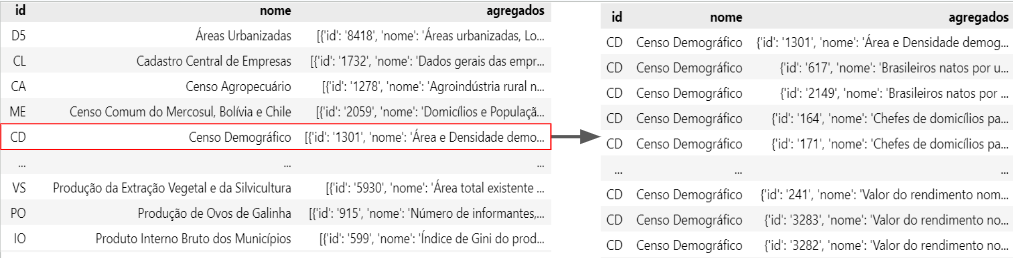
\includegraphics[width=\textwidth]{files/img/exploding_table.png}    \caption{Exemplo do uso do método \lstinline{pandas.DataFrame().explode()}. Fonte: Dados do autor (2023).}
    \label{fig:exploding-df}
\end{figure}

    Nota-se que os valores ``explodidos'' continuam aninhados, portanto nesse caso foi necessário reaplicar a função \lstinline{unnest_json()} de modo a separar adequadamente os dados. O processo completo é uma sequência de aplicação dessas duas funções conforme o necessário até termos um \textit{DataFrame} completamente desaninhado.

    Das 17 APIs disponíveis, foram carregados dados das APIs de localidades, países, agregados e metadados. A API de localidades retorna as informações referentes aos identificadores geográficos do país definidos pelo IBGE, utilizados para identificar a área na qual foram coletados em praticamente todas as pesquisas do órgão. Esse serviço de dados possui ao todo quatro possíveis requisições nas quais os dados são separados por distritos, subdistritos, região metropolitana e região integrada de desenvolvimento. Os conjuntos de dados derivados podem ser juntados entre si através do identificador mais específico presentes nelas, sendo o ID do distrito nas duas primeiras e o id do município nas outras duas.

    Contendo 34 indicadores socioeconômicos dos 193 países membros da Organização das Nações Unidas (ONU) a API de países é a única que não utiliza apenas dados coletados pelo próprio IBGE e que também possui traduções em Espanhol e Inglês. Como uma requisição comum solicita a especificação dos países e/ou das variáveis desejadas, a estratégia adotada foi primeiramente obter todos os códigos distintos de países para posteriormente realizar uma requisição para cada país contendo todos os possíveis indicadores e concatenando todos os resultados em um único conjunto de dados. O código completo pode ser encontrado no \textit{listing} \ref{apend-code}.\ref{lst:api-paises}.

    A carga mais elaborada foi a de agregados, onde foi necessário primeiramente selecionar os IDs dos agregados, totalizando 8442 agregados de 68 pesquisas, cada qual contendo diversas variáveis e séries temporais. Então, obtidos os identificadores, foram requisitados à API os metadados de cada pesquisa. Tendo os dados de nível e o ID do agregado foi então possível usar a URL `https://servicodados.ibge.gov.br/api/v3/agregados/
    \{agregado\}/variaveis?localidades=\{nivel\}[all]', onde \verb|{agregado}| e \verb|{nivel}| são parâmetros passados conforme os metadados obtidos. 
    
    O resultado da requisição acima, transformado em \textit{DataFrame} é o mostrado na figura \ref{fig:tabela-agregado-pt1}. A coluna mais importante é de resultados, que irá conter duas listas de valores: classificações, contendo metadados acerca da variável, e, novamente, resultados, que por sua vez também contem listas, mas dessa vez com as séries dos valores numéricos. 
    
    Aplica-se então o método \verb|explode()| ao \textit{DataFrame} até termos os valores das séries distribuídos em uma coluna por ano, que, para normalizar a tabela, é executado o método \verb|melt()| para criar-se uma coluna de período e outra de valor. O resultado final é um conjunto de dados com as colunas variável, unidade, id, nome e nível geográfico da localidade (p. ex. Município, UF, \textit{etc.}), ano e valor.

\begin{figure}[ht]
    \centering
    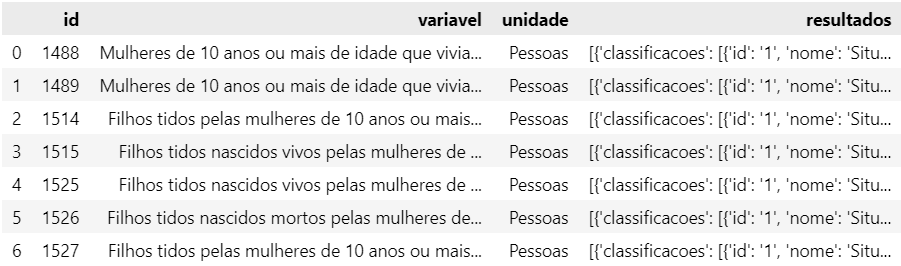
\includegraphics[width=\textwidth]{files/img/tabela_agregado_pt1.png}
    \caption{Tabela de dados após primeira requisição para a carga dos agregados. Fonte: Dados do Autor (2023).}
    \label{fig:tabela-agregado-pt1}
\end{figure}



    


\section{Microdados do Censo Demográfico}
\label{sec-microdados}

    Os dados fornecidos pela API de agregados consistem essencialmente na consolidação das respostas individuais de cada um dos entrevistados durante o processo de recenseamento de acordo com critérios locacionais, com seu menor grau de agregação sedo município. Tais informações são organizadas em um formato denominado pelo IBGE como microdados e são disponibilizados através do portal de produtos estatísticos da instituição\footnote{Para mais detalhes, consulte <\url{www.ibge.gov.br/estatisticas/todos-os-produtos-estatisticas.html}>. Acesso em 03 out. 2023}, estando disponibilizados em diversas pastas compactadas em formato \textit{.zip} que contém os arquivos de texto nos quais se encontram os dados. No entanto, os dados daqueles arquivos não estão imediatamente prontos para a utilização tal qual uma planilha ou um arquivo CSV, mas sim em um formato comprimido, onde os valores categóricos são codificados através de identificadores (IDs) numéricos, enquanto valores que originalmente possuíam casas decimais tem seus pontos flutuantes removidos. Dessa forma, os dados se apresentam conforme ilustrado pela figura \ref{fig:exemplo-microdado}:

\begin{figure}[ht]
    \centering
    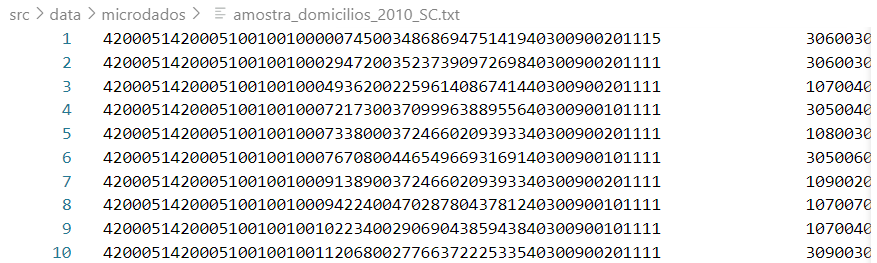
\includegraphics[width=\textwidth]{files/img/exemplo_microdado.png}
    \caption{Exemplo de microdados: primeiras 10 linhas da pesquisa de Domicílios do Censo de 2010 no estado de Santa Catarina. Fonte: Dados do Autor (2023)\protect\footnotemark.}
    \label{fig:exemplo-microdado}
\end{figure}
\footnotetext{\textit{Printscreen} do arquivo de microdados da amostra de domicílios do Estado de Santa Catarina, Censo de 2010.}

    Juntamente com os microdados, é fornecido uma planilha no formato \textit{Open Document Spreadsheet} (ODS) ou Excel que descreve o que cada caractere do arquivo significa, relacionando as categorias e identificadores e a formatação referente às casas decimais das variáveis numéricas. 
    
    Tomando como exemplo a amostra da pesquisa de domicílios do Censo Demográfico de 2010, o arquivo de \textit{layout}
    \footnote{Arquivo /Documentação/Layout/Layout\_microdados\_amostra.xls. Download em: <\url{ftp.ibge.gov.br/Censos/Censo_Demografico_2010/Resultados_Gerais_da_Amostra/Microdados/Documentacao.zip}>. Acesso em 03 out. 2023.} (exemplificado na figura \ref{fig:layout-domi}), temos que as duas primeiras posições do arquivo referem-se variável V0001 à UF, cujo valor 42 corresponde ao Estado de Santa Catarina. Outro exemplo significativo é a variável numérica V0010, Peso Amostral, engloba os dígitos da posição 29 até 44, sendo os 3 primeiros (coluna INT) os dígitos anteriores ao ponto decimal, e as 13 subsequentes sendo as casas de precisão após a vírgula (coluna DEC).

\begin{figure}[ht]
    \centering
    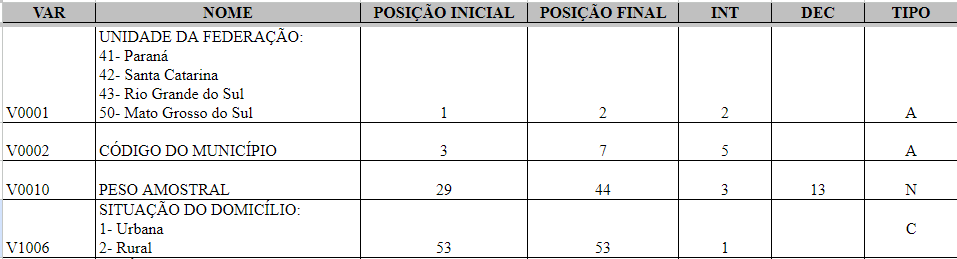
\includegraphics[width=\textwidth]{files/img/layout amostra domicilios 2010.png}
    \caption{Recorte da planilha de \textit{layout} da pesquisa de domicílios do Censo Demográfico de 2010. Fonte: Dados do Autor (2023)\protect\footnotemark.}
    \label{fig:layout-domi}
\end{figure}
\footnotetext{Com base na planilha de \textit{layout} da amostra de domicílios do Censo Demográfico de 2010.}

    Variáveis padrões contidas nas pesquisas são as referentes à localização geográfica como município, UF e área de ponderação, assim como o peso amostral, que por sua vez é uma medida de representatividade daquela resposta dentro do escopo da pesquisa.

    Os arquivos de microdados ficam disponíveis através da URL <\url{www.ibge.gov.br/estatisticas/sociais/trabalho/22827-censo-demografico-2022.html?edicao=37225&t=microdados}>, separados por Estado e por Censo, hoje\footnote{Considerando o último acesso em novembro de 2023.} estando disponíveis os microdados Censos de 2000 e 2010 no \textit{website}. Com o intuito de facilitar o processo de baixar os arquivos, foi codificado um \textit{script python}\footnote{Código completo no arquivo download-arquivos-microdados.ipynb, disponível em: <\url{github.com/GDevigili/TCC-IBGE/blob/main/src/notebooks/download-arquivos-microdados.ipynb}>} para tal, que realiza o \textit{download} de todos os arquivos \verb|.zip|, descompacta eles e então os renomeia, de modo a padronizar os nomes dos arquivos de ambas pesquisas e separar as diferentes amostras, além de separar arquivos de dados dos arquivos auxiliares que estão inclusos nos diretórios compactados. Vale ressaltar que os arquivos não processados não foram incluídos no repositório por conta do limite máximo de 100 megabytes (MB) que o \textit{Github} impõe para os arquivos.

    Após extraídos os \verb|zip|s, tem-se uma coleção de arquivos de texto (de extensão \verb|.txt|) contendo os microdados codificados como na figura \ref{fig:exemplo-microdado}. Para transformá-los em dados utilizáveis, os microdados precisam ser associados aos respectivos valores, descritos no arquivo de \textit{layout}.

    Inicialmente, tentou-se fazer tal ``tradução'' via \textit{python}\footnote{Código completo no arquivo translate-microdata.ipynb, disponível em <\url{github.com/GDevigili/TCC-IBGE/blob/main/src/notebooks/old-notebooks/2-translate-microdata.ipynb}>}, manualmente programando tal a associação dos IDs com suas respectivas \textit{labels}. Primeiramente destrinchando o arquivo de descrição das variáveis em pares chave-valor e dividindo os números dos microdados em colunas de acordo com as respectivas posições inicial e final, armazenando ambos os resultados deste pré-processamento em \verb|DataFrame| da biblioteca \verb|pandas|. Tendo em mãos os objetos necessários, foi iterado através de cada linha e coluna, substituindo os identificadores por suas respectivas \textit{labels}.

    Porém, o custo computacional de se processar os dados dessa forma, ainda mais utilizando uma linguagem \textit{python}, conhecida por um tempo de execução elevado, além da presença de \textit{bugs} no código devido ao funcionamento de algumas estruturas de dados da \verb|pandas|, foi optado por realizar o mesmo trabalho utilizando o \textit{software Stata} (em sua versão 18.0), que possui funções já implementadas para o processamento de arquivos como os do IBGE.

    Com comandos da linguagem própria do \textit{Stata}, é possível fazer a mesma associação de identificadores e labels com alguns poucos comandos, para então gerar um arquivo de dados de extenção \verb|.dta| que posteriormente poderá ser utilizado como \textit{dataset}. Por exemplo, no \textit{Listing} \ref{lst:do-file-sample} definimos a posição das variáveis, sua tipagem, respectivas \textit{labels} e possíveis valores, nos casos de colunas categóricas, ou formatação, em caso de colunas numéricas.

    % De modo a preparar os microdados para que estes possam ser utilizados, foi utilizado o \textit{software} Stata (em sua versão 18.0) para associar os IDs e respectivos valores descritos no arquivo de \textit{layout} e então gerar um arquivo de dados que posteriormente poderá ser utilizado como \textit{dataset}. 
    % Com comandos do Stata é possível definir a posição em que se encontram as informações de cada variável, sua tipagem, suas \textit{labels} e respectivos pares chave e valor, para então o arquivo de dados ser processado, que é exemplificado pelo \textit{Listing} \ref{lst:do-file-sample} a seguir:

\begin{lstlisting}[float = ht, label={lst:do-file-sample},language=Stata, caption=Exemplo de comandos Stata utilizados para``traduzir'' os microdados.]
* Define as posições onde se encontram cada dado
quietly infix               ///
  byte		V1006		53-53		  ///
  double		V6204		82-84		///
using `"amostra_domicilios_2010_RJ.txt"', clear
* Define a formatação dos dados numéricos
* Neste caso,  o dado deve assumir a formatação 0000.0
format V6204 %04.1f
* Define as labels para os dados
label var V1006		`"SITUAÇÃO DO DOMICÍLIO"'
label var V6204		`"DENSIDADE DE MORADOR / DORMITÓRIO  "'
* Define os pares chave-valor para cada variável
label define V1006_lbl 1 `" Urbana"', add
label define V1006_lbl 2 `" Rural"', add
* Associa os valores da variável V1006 com os pares chave-valor armazenados em V1006_lbl
label values V1006 V1006_lbl
\end{lstlisting}

    O código exemplificado nada mais é que um pequeno recorte do arquivo\footnote{Arquivo\ amostra\_domicilios\_2010.do, disponível em <\url{https://github.com/GDevigili/TCC-IBGE/blob/main/src/do-files/amostra_domicilios_2010.do}>} completo da pesquisa de domicílios, que conta com 76 variáveis e mais de 6 mil \textit{labels}, em sua maioria referentes à localização geográfica da coleta da amostra, já que estão inclusos mais de 5 mil municípios e 500 microrregiões.

    Para não ser necessário definir manualmente cada uma das variáveis, aproveitou-se parte do código que seria descartada na tentativa de realizar a ``tradução'' dos microdados via \textit{python} e se utilizou do processamento da tabela de \textit{layout} para gerar um \textit{DataFrame} contendo os pares chave-valor utilizados para mapear via comando \verb|label define| as possíveis \textit{labels} de cada uma das colunas utilizando um \textit{script} que itera sobre a tabela processada.

    Além disso, como os códigos de município, micro e mesorregião ficam em planilhas auxiliares, foi optado por utilizar dos identificadores de localidade coletados via API para associar os respectivos códigos no \textit{Dofile} que seria executado no \textit{Stata} para gerar o conjunto de dados. A única transformação necessária foi o uso de uma coluna auxiliar que juntava o código da UF com os códigos de município e regiões, já que a API utiliza chaves concatenadas como identificadores.

    Após gerado o \textit{Dofile} através do \textit{script} \textit{python} descrito acima, só é necessário carregar o arquivo no \textit{Stata} e executá-lo, por fim salvando o novo arquivo de dados. Caso aberto através de um editor de texto, o arquivo \verb|.dta| se parece com o arquivo de microdados, porém carrega as configurações de \textit{label} e formatação que foram definidas anteriormente. Para a leitura do arquivo em um amiente diferente do \textit{software} estatístico, é necessário um leitor específico. Além disso é possível a conversão do \verb|.dta| para formatos mais comuns de armazenamento de dados, como \textit{Excel} ou arquivos de texto com delimitadores como \textit{Comma} ou \textit{Tab separated values} (CSV e TSV respectivamente). 
    
    % Como facilitador para tal associação de pares chave-valor, foi desenvolvido um código \textit{python}\footnote{Código disponível em <\url{https://github.com/GDevigili/DW-IBGE/blob/main/src/notebooks/gera-script-stata.ipynb}>.} que gera um \textit{script} para ser utilizado pelo Stata para o processamento  ``tradução'' dos microdados. 
   
    % Primeiramente, por meio das colunas de posição inicial e final, foram mapeados os caracteres que representam cada uma das variáveis do conjunto de dados, então foi adicionada a formatação adequada para os dados numéricos com o comando \verb|format|. Posteriormente são definidos os nomes das colunas com o comando \verb|label define| e então associados os pares chave-valor, extraídos de um \verb|DataFrame| pré processado com os dados presentes no arquivo de \textit{layout}. Os valores correspondentes aos municípios, microrregiões, mesorregiões e regiões metropolitanas se encontram em arquivos auxiliares, porém foi optado por utilizar a própria API de localidades para obter os respectivos valores já que o trabalho para a extração de dados já havia sido realizado anteriormente.


\chapter{Estudo de Caso: Acesso à água encanada no Estado do Rio de Janeiro}

    Exemplificando um possível caso de uso dos conjuntos de dados estudados, será realizada uma análise da distribuição de água encanada no Estado do Rio de Janeiro.

    Para o carregamento do arquivo de dados do \textit{Stata} no \textit{python}, foi necessário abrir os arquivos na forma de um objeto do tipo \verb|StataReader| que permite o acesso às \textit{labels} definidas na execução do \textit{Dofile} para posterior aplicação no conjunto de dados. A carga completa se encontra no \textit{listing} \ref{lst:read-stata}. 
    
    A variável utilizada para o cálculo do valor foi a coluna ``V0209: Abastecimento de Água, Canalização'' da amostra de domicílios do Censo de 2010. Foram consideradas no cálculo do percentual as respostas ``Sim, em pelo menos um cômodo'' e ``Sim, só na propriedade ou terreno'' e a ponderação da representatividade da resposta foi dada através da coluna de peso amostral (V0010). Por se tratarem de dados com uma média de 98.74\% e mediana em 99.54\%, uma escala contínua deixaria o mapa gerado de difícil interpretação, então foi optado por subdividir os dados em 5 categorias: Menor que 80\%, entre 80\% e 90\%, entre 90\% e 95\%, entre 95\% e 98\% e entre 98\% e 100\%.

    Analisando unicamente as 200 áreas de ponderação do município do Rio de Janeiro através da figura \ref{fig:box-rio}, fica claro que menos de 5\% das áreas da capital possuem menos de 95\% dos domicílios com água encanada.

\begin{figure}[ht]
    \centering
    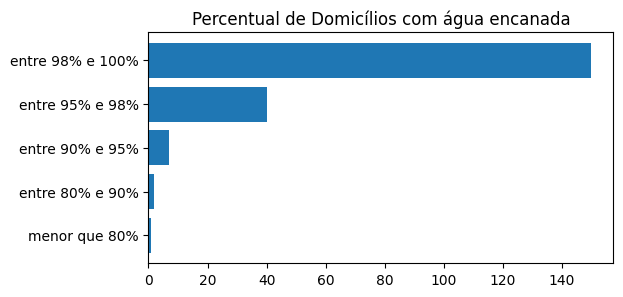
\includegraphics[width=0.8\textwidth]{files/img/boxplot rio 2.png}
    \caption{\textit{Boxplot} do percentual de domicílios com água canalizada no município do Rio de Janeiro. Fonte: Dados do Autor (2023)\protect\footnotemark.}
    \label{fig:box-rio}
\end{figure}
\footnotetext{Com base nos microdados da amostra de domicílios de 2010 do Estado do Rio de Janeiro.}
    
    Para a criação de uma visualização (Figura \ref{fig:mapa-rj}) referente aos dados, foi utilizado um arquivo \textit{Shapefile}\footnote{Arquivos \textit{shapefile} referentes aos Estados brasileiros disponíveis em: \url{https://geoftp.ibge.gov.br/organizacao_do_territorio/malhas_territoriais/malhas_de_setores_censitarios__divisoes_intramunicipais/censo_2010/setores_censitarios_shp/}. O arquivo utilizado foi de extensão \protect\verb|.shp da pasta compactada \verb|rj\_setores\_censitarios.zip}}, que são arquivos vetoriais que armazenam forma e atributos de localizações geográficas \cite{arcgis}. Através a biblioteca \textit{GeoPandas} é possível manipular esse conjunto de dados geográficos, juntá-los com outros \textit{datasets} e também gerar gráficos. Acrescentando as porcentagens calculadas com os microdados ao \textit{dataframe}, foi utilizado o método \verb|plot()| com algumas configurações comuns da biblioteca \verb|matplotlib| para exibir as categorias acima citadas. 


\begin{figure}[ht]
    \centering
    \includegraphics[width=0.9\textwidth]{files/img/mapa água micro.png}
    \caption{Mapa do percentual de domicílios com água encanada no Estado do Rio de Janeiro com base nos microdados da amostra de domicílios. Fonte: Dados do Autor (2023)\protect\footnotemark}
    \label{fig:mapa-rj}
\end{figure}
\footnotetext{Com base nos microdados da amostra de domicílios de 2010 do Estado do Rio de Janeiro.}

    Como comparativo, foi também utilizada a base de agregados, mais especificamente a variável 1000096: ``Existência de água canalizada'' agregado no nível de localidade de município (N6). A variável em questão já está calculada em percentual do total e o valor utilizado foi, novamente, a soma das respostas afirmativas à questão. Comparando o gráfico com os dados da API lado à lado com o da figura \ref{fig:mapa-rj}, podemos observar pequenas variações de valor:

\begin{figure}[ht]
    \centering
    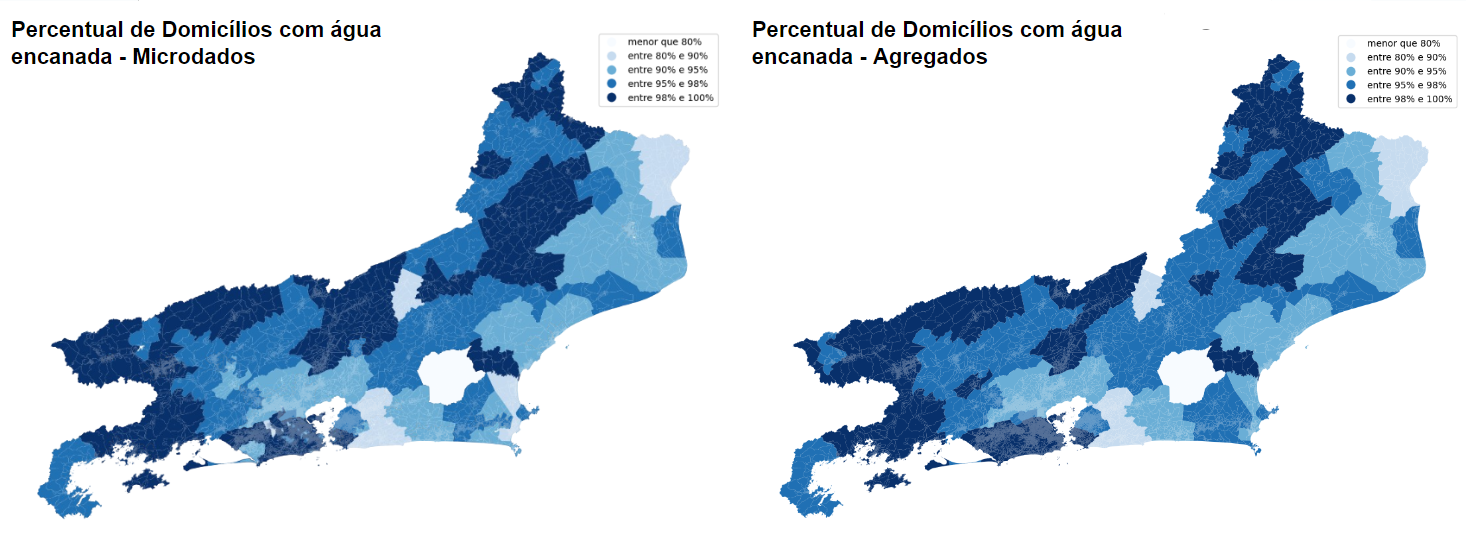
\includegraphics[width=\textwidth]{files/img/mapa rj agua.png}
    \caption{Comparação entre os mapas de percentual de domicílios com água canalizada no RJ. Na esquerda o gráfico com base nos microdados e na direita com base nos dados agregados da API. Fonte: Dados do Autor (2023).}
    \label{fig:mapa-rj-compara}
\end{figure}

    Pouco muda entre um gráfico e outro, já que eles representam em tese a mesma coisa, mas algumas poucas variações mostram como o nível de detalhe dos microdados revela informações que são perdidas no gráfico de agregados\footnote{Gráfico em tamanho maior na imagem \ref{fig:mapa-rj-agg} do apêndice \ref{sec-ap-img}}, como na região mais ao norte do Estado, que aparenta ter mais regiões com água encanada porém a agregação ``mascara'' certos pontos menores que entram na categoria ``entre 95\% e 98\%'' ao invés da categoria superior.
    
    Uma análise mais minuciosa pode ser feita visualizando apenas a capital do Estado, como na \ref{fig:mapa-mun-rio}. Com os microdados, se revela que mesmo em um município com mais de 99\% de água encanada, ainda existem áreas como os bairros como Guaratiba e Bangu com um acesso consideravelmente menor ao serviço que tiveram suas amostras ofuscadas pelo restante da cidade.

\begin{figure}[ht]
    \centering
    \includegraphics[width=0.9\textwidth]{files/img/mapa rio água.png}
    \caption{Percentual de Domicílios com água encanada no município do Rio de Janeiro. Fonte: Dados do Autor (2023).}
    \label{fig:mapa-mun-rio}
\end{figure}


\chapter{Conclusão}

Os dados do Instituto Brasileiro de Geografia e Estatística são de enorme valor para diversos setores do país, tanto no âmbito público quanto privado. Tais dados podem ser coletados em dois formatos distintos, um em JSON via API de serviço de dados do instituto e o outro em arquivos de texto codificados de acordo com identificadores presentes em um arquivo de \textit{layout}. Em ambos os formatos, após certo processamento e transformação, é possível

Com base na análise das APIs fornecidas do IBGE, conclui-se que 

% Com base na análise das APIs fornecidas pelo IBGE, conclui-se que essas ferramentas oferecem uma gama diversificada de dados que abrangem desde informações geográficas até indicadores socioeconômicos. Com um total de 17 APIs, destacam-se a de Agregados, que compreende uma extensa variedade de dados de pesquisas, e a de Localidades, que disponibiliza códigos e informações sobre diferentes níveis de localidade, como municípios e regiões.

% A utilização dessas APIs é facilitada por meio de \textit{Uniform Resource Locators} (URLs), permitindo a geração de requisições com bibliotecas como \textit{requests} do \textit{Python}. A ferramenta de \textit{Querie Builder} integrada à plataforma contribui para a construção eficiente dessas URLs, simplificando o processo de obtenção de dados no formato \textit{Javascript Object Notation} (JSON).

% No entanto, a complexidade intrínseca à estrutura JSON pode dificultar a análise direta dos dados. Visando a simplicidade na criação de consultas, foi aplicado um processo de \textit{unnesting} à \textit{string} de resultados das requisições, permitindo a normalização dos dados para análises mais eficazes.

% O exemplo prático de \textit{unnesting} foi demonstrado com a API de localidades, onde a transformação dos dados JSON em um formato tabular facilitou a compreensão e análise. Além disso, a abordagem de lidar com elementos em formato de lista foi explorada, utilizando métodos como \lstinline{pandas.DataFrame().explode()}.

% No processo de carga e análise de dados, foram exploradas três APIs específicas: Localidades, Países e Agregados. Cada uma delas apresentou desafios únicos, desde a manipulação de identificadores geográficos até a elaborada extração de indicadores socioeconômicos e agregados.

% Ao finalizar as análises, conclui-se que as APIs do IBGE oferecem uma rica fonte de dados, abrindo oportunidades para estudos detalhados em diversas áreas, como geografia, economia e demografia. A abordagem adotada para lidar com a complexidade dos dados demonstrou ser eficaz, proporcionando uma base sólida para análises mais aprofundadas e insights valiosos.


% \item Estudar diferentes estratégias de coleta de dados censitários do IBGE;
%     \item Carregar os dados do IBGE via API e processá-los de forma a reestruturar eles em formato tabular;
%     \item Codificar um \textit{script} capaz de ler e associar \textit{labels} aos respectivos microdados de modo a gerar um arquivo de dados do \textit{Stata};
%     \item Demonstrar o uso de ambos conjuntos de dados através de um estudo de caso, demonstrando as diferenças de abrangência e utilização dos dois formatos estudados (API e microdados), gerando visualizações e estatísticas básicas.

% -----------------------------------
% ELEMENTOS PÓS-TEXTUAIS
% -----------------------------------
\postextual
% ----------------------------------

%\bibliography{biblio}
\printbibliography

%\glossary

% ----------------------------------------------------------
% Apêndices
% ----------------------------------------------------------

% ---
% Inicia os apêndices
% ---
\begin{apendicesenv}

% % Imprime uma página indicando o início dos apêndices
\partapendices

\setlength{\absparsep}{18pt} 
\begin{apendicesenv}

\chapter{Códigos}

\end{apendicesenv}

\end{apendicesenv}

% ---

% ----------------------------------------------------------
% Anexos
% ----------------------------------------------------------

% \begin{anexosenv}

% \partanexos

% \end{anexosenv}

%---------------------------------------------------------------------
% ÍNDICE REMISSIVO
%---------------------------------------------------------------------
% \phantompart
% \printindex

\end{document}